\chapter{Termo de Abertura do projeto}

\section{EAP}
\section{Lista É/Não é}
\subsection{É}
\subsection{Não é}
\section{Requisitos}
\subsection{Eletrônica}
\subsection{Energia}
\subsection{Estrutura}
\subsection{Software}
\section{\emph{Stakeholders}}
\section{Organização do projeto}

\subsection{Recursos humanos}
  
  De modo a ter uma melhor organização, a equipe foi dividida em subgrupos, onde cada subgrupo tem um gerente técnico, além disso a equipe também conta com um gerente de qualidade e um coordenador geral. Na Figura %\ref{fig:organograma}
 mostra o organograma da equipe e o nome de cada integrante por função.
 
\begin{figure}[h]
\centering
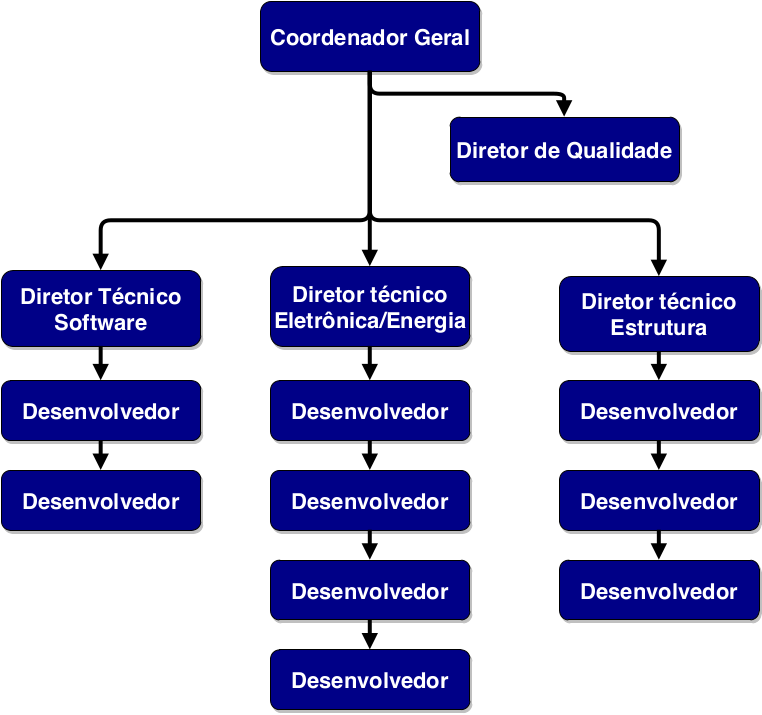
\includegraphics[scale = 1]{organograma.pdf}
\caption{.}\label{fig:organogram}
\end{figure} 
  
\subsection{Gerenciamento do projeto} 



\section{Cronograma de atividades}
\section{Milestones Identificados}
\section{Estimativa de custos}
\section{Viabilidades financeira}
\section{Levantamento de riscos}
